\chapter{SystemC Modelling and Implementation}
\label{chap:systemc_modelling}

\section{Introduction}

This chapter presents the comprehensive SystemC implementation of our pipelined floating-point processor, covering both the overall processor architecture and the detailed implementation of IEEE 754 floating-point arithmetic units. The implementation translates the architectural design into executable SystemC code that maintains IEEE 754 compliance while ensuring synthesis compatibility with Intel SystemC-to-SystemVerilog tools.

The key challenge addressed is maintaining IEEE 754 compliance while ensuring the SystemC code translates to efficient, synthesizable hardware. Our approach balances performance, area efficiency, and timing constraints through carefully designed pipeline architectures and optimized arithmetic units.

\section{SystemC Modelling Approach}
\label{sec:systemc_approach}

SystemC provides a C++ based hardware description and modelling language that bridges the gap between software and hardware design. As a class library built on standard C++, it extends the language with hardware constructs including:

\begin{itemize}
    \item \textbf{Modules:} Act as hardware building blocks that represent distinct parts of the system and hide internal details behind interfaces
    \item \textbf{Ports:} Define communication interfaces between modules
    \item \textbf{Signals:} Act as wires between modules carrying data from one port to another, mimicking hardware connections
    \item \textbf{Processes:} Independent workers inside modules that run simultaneously, triggered by signals, clocks or events
    \item \textbf{Events:} Help synchronize different parts of design, ensuring proper timing
    \item \textbf{Clocks:} Provide timing reference for synchronous logic with flip-flops, registers and state machines updating on clock edges
\end{itemize}

\subsection{Cycle-Accurate RTL Abstraction}
\label{subsec:cycle_accurate}

For this pipeline implementation, we employ a cycle-accurate RTL-like abstraction level that models the behavior of our processor where every clock cycle matters, and pipeline stages are modelled precisely. This approach allows us to:

\begin{itemize}
    \item Observe how instructions flow through the pipeline
    \item Model data dependencies and control flow logic accurately
    \item Verify functional correctness with exact timing and no approximations
    \item Generate synthesizable RTL that directly maps to hardware
\end{itemize}

The model behaves like Verilog/VHDL making actual chip design straightforward. While higher abstraction levels could improve simulation speed, the cycle-accurate approach was necessary to validate our processor architecture and ensure synthesis compatibility.

\section{SystemC Synthesis Constraints and Design Methodology}
\label{sec:synthesis_constraints}

The Intel SystemC compiler imposes specific requirements for synthesizable code that influenced our entire design methodology:

\begin{itemize}
    \item \textbf{Thread Structure}: Use \texttt{SC\_CTHREAD} instead of \texttt{SC\_METHOD} for clocked processes
    \item \textbf{State Management}: Explicit state transitions with \texttt{while(true)} loops and \texttt{wait()} statements
    \item \textbf{Reset Handling}: Automatic reset using \texttt{reset\_signal\_is()} declarations
    \item \textbf{Data Types}: Only synthesizable types (\texttt{sc\_uint}, \texttt{bool}) - no floating-point types
    \item \textbf{Pipeline Registers}: Explicit pipeline stage separation with proper timing
\end{itemize}

Each \texttt{wait()} statement corresponds to a clock boundary, and code between consecutive \texttt{wait()} statements represents combinational logic within a single clock cycle.

\section{SystemC Module Hierarchy}
\label{sec:module_hierarchy}

Our SystemC implementation follows a hierarchical structure combining the five-stage pipeline with specialized IEEE 754 arithmetic units. The processor implementation consists of the following primary modules:

\begin{itemize}
    \item \textbf{Instruction Fetch Unit}: Program counter management and instruction memory access
    \item \textbf{Decode Unit}: Instruction decoding and register file access
    \item \textbf{Execute Unit}: Floating-point operation execution with dedicated arithmetic units
    \item \textbf{Memory Access Unit}: Pipeline register stage for memory operations
    \item \textbf{Writeback Unit}: Result integration into processor state
    \item \textbf{Arithmetic Units}: IEEE 754 compliant adder, subtractor, multiplier, and divider
    \item \textbf{Supporting Components}: Instruction memory and register file
\end{itemize}

Each stage connects to the next through registers and ports, forming the complete processor data path. Each process typically has two main sections: a reset section for initialization and an infinite loop where communication and computation occur.

\begin{figure}[htbp]
    \centering
    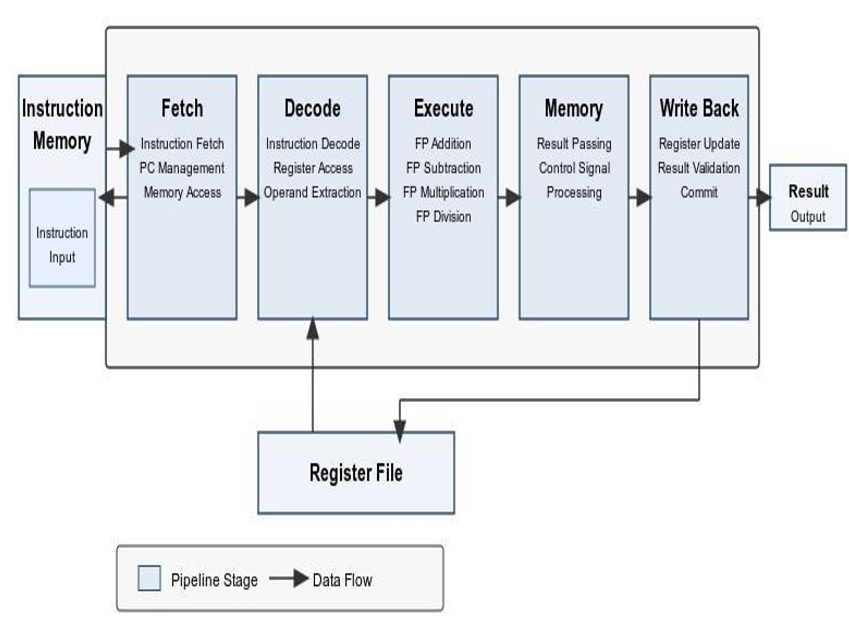
\includegraphics[width=0.8\textwidth]{pipeline_diagram.png}
    \caption{SystemC module hierarchy of the pipelined floating-point processor}
    \label{fig:systemc_hierarchy}
\end{figure}



\section{Interface Definitions and Communication}
\label{sec:interface_definitions}

Each module defines clear interfaces using SystemC ports and signals. The primary pipeline interface includes:

\begin{lstlisting}[caption={Pipeline Stage Interface}]
// Input ports
sc_in<bool> clk;                    // System clock
sc_in<bool> reset;                  // Active-high reset
sc_in<bool> stall;                  // Stall signal
sc_in<sc_uint<32>> instruction_in;  // Instruction input
sc_in<bool> valid_in;               // Validity flag for input

// Output ports
sc_out<sc_uint<32>> result_out;     // Operation result
sc_out<sc_uint<5>> rd_out;          // Destination register
sc_out<bool> reg_write_out;         // Register write enable
sc_out<bool> valid_out;             // Validity flag for output
sc_out<sc_uint<32>> instruction_out; // Instruction forwarded
\end{lstlisting}

These standardized interfaces ensure consistent communication between pipeline stages, facilitating modular design and verification.

\section{IEEE 754 Arithmetic Units Implementation}
\label{sec:arithmetic_units}

The heart of our floating-point processor lies in the IEEE 754 compliant arithmetic units. Each unit follows synthesis-compatible design patterns while maintaining full standard compliance.

\subsection{IEEE 754 Addition/Subtraction Algorithm}
\label{subsec:ieee754_addition}

\subsubsection{Algorithm Overview}

IEEE 754 addition/subtraction follows these steps:
\begin{enumerate}
    \item Extract sign, exponent, and mantissa from both operands
    \item Align mantissas by shifting the smaller operand
    \item Perform mantissa addition or subtraction based on signs
    \item Normalize the result and handle overflow/underflow
\end{enumerate}

\subsubsection{3-Stage Implementation}

The addition/subtraction unit implements a 3-stage process optimized for synthesis compatibility:

\textbf{Stage 1: Operand Extraction}
\begin{lstlisting}[caption=Extraction Stage Implementation]
void extract_stage() {
    // Reset outputs
    sign_a_reg2.write(0);
    // ... other resets
    wait();
    
    while (true) {
        // Extract IEEE 754 components
        bool sign_a = A_reg1.read()[31];
        sc_uint<8> exp_a = A_reg1.read().range(30, 23);
        sc_uint<24> mant_a;
        
        if (exp_a == 0) {
            mant_a = (sc_uint<24>)((sc_uint<1>(0), 
                     A_reg1.read().range(22, 0)));
        } else {
            mant_a = (sc_uint<24>)((sc_uint<1>(1), 
                     A_reg1.read().range(22, 0)));
        }
        
        // Register for next stage
        sign_a_reg2.write(sign_a);
        exp_a_reg2.write(exp_a);
        mant_a_reg2.write(mant_a);
        wait();
    }
}
\end{lstlisting}

\textbf{Stage 2: Addition/Subtraction Logic}
\begin{lstlisting}[caption=Addition Core Logic]
void add_stage() {
    // Reset state
    wait();
    
    while (true) {
        // Determine larger operand for alignment
        if (exp_a_reg2.read() > exp_b_reg2.read()) {
            diff = exp_a_reg2.read() - exp_b_reg2.read();
            tmp_mantissa = mant_b_reg2.read() >> diff;
            
            if (sign_a_reg2.read() == sign_b_reg2.read()) {
                // Same signs: addition
                out_mantissa = mant_a_reg2.read() + tmp_mantissa;
            } else {
                // Different signs: subtraction
                out_mantissa = mant_a_reg2.read() - tmp_mantissa;
            }
        }
        // Handle other cases...
        wait();
    }
}
\end{lstlisting}

\textbf{Stage 3: Normalization}
\begin{lstlisting}[caption=Normalization Stage]
void normalize_stage() {
    O.write(0);
    wait();
    
    while (true) {
        if (norm_mantissa[24]) {
            // Overflow: shift right, increment exponent
            norm_exponent = norm_exponent + 1;
            norm_mantissa = norm_mantissa >> 1;
        } else if (norm_mantissa[23] == 0) {
            // Underflow: count leading zeros, shift left
            for (lz = 0; lz < 24 && norm_mantissa[23-lz] == 0; lz++);
            norm_exponent = norm_exponent - lz;
            norm_mantissa = norm_mantissa << lz;
        }
        
        result = (sign, norm_exponent, norm_mantissa.range(22,0));
        O.write(result);
        wait();
    }
}
\end{lstlisting}

\subsection{IEEE 754 Multiplication Algorithm}
\label{subsec:ieee754_multiplication}

\subsubsection{Algorithm Design}

Multiplication requires additional stages due to the complexity of 24×24-bit mantissa multiplication.

The key algorithmic steps include:
\begin{enumerate}
    \item \textbf{Operand Preparation}: Extract components and handle special cases (NaN, infinity, zero)
    \item \textbf{Sign Calculation}: XOR operation on sign bits  
    \item \textbf{Exponent Addition}: Add biased exponents and adjust for bias
    \item \textbf{Mantissa Multiplication}: 24×24 bit multiplication including implicit leading ones
    \item \textbf{Normalization \& Rounding}: Final result adjustment with IEEE 754 compliance
\end{enumerate}
\begin{lstlisting}[caption=Multiplication and Exponent Addition]
void mult_cycle2_exp_stage() {
    wait(); // Reset state
    
    while (true) {
        // Complete 24x24 bit multiplication
        sc_uint<48> full_mult_result = 
            mant_a_reg3.read() * mant_b_reg3.read();
        
        // Calculate result sign (XOR)
        bool result_sign = sign_a_reg3.read() ^ sign_b_reg3.read();
        
        // Add exponents and subtract bias
        sc_uint<9> temp_exp = exp_a_reg3.read() + exp_b_reg3.read();
        sc_uint<9> result_exp = (temp_exp >= 127) ? 
                                temp_exp - 127 : 0;
        
        result_sign_reg4.write(result_sign);
        result_exp_reg4.write(result_exp);
        mult_result_reg4.write(full_mult_result);
        wait();
    }
}
\end{lstlisting}

\textbf{Stage 5: Normalization \& Rounding}
\begin{lstlisting}[caption=Multiplication Normalization]
void normalize_round_stage() {
    O.write(0);
    wait();
    
    while (true) {
        sc_uint<48> mult_result = mult_result_reg4.read();
        
        // Normalization based on result magnitude
        if (mult_result[47]) {
            // Result is 1.xxx (overflow)
            final_mantissa = mult_result.range(46, 24);
            final_exponent = exp_result + 1;
        } else if (mult_result[46]) {
            // Result is 0.1xxx (normal)
            final_mantissa = mult_result.range(45, 23);
            final_exponent = exp_result;
        } else {
            // Underflow: find first significant bit
            // Shift left and adjust exponent accordingly
        }
        
        result = (sign_result, final_exponent, final_mantissa);
        O.write(result);
        wait();
    }
}
\end{lstlisting}

\subsection{IEEE 754 Division Algorithm}
\label{subsec:ieee754_division}

\subsubsection{Algorithm for Iterative Division}

Division is the most complex operation, requiring an iterative division algorithm. The key algorithmic steps include:

\begin{enumerate}
    \item \textbf{Preparation}: Input validation and special case handling
    \item \textbf{Sign Determination}: XOR operation on operand signs
    \item \textbf{Exponent Subtraction}: Subtract divisor exponent from dividend exponent
    \item \textbf{Iterative Division}: Restoring division algorithm for significands
    \item \textbf{Normalization}: Final result formatting with exception detection
\end{enumerate}

\textbf{Division Iteration Implementation:}
\begin{lstlisting}[caption=Division Iteration Stage]
void division_stage1() {
    // Reset state
    wait();
    
    while (true) {
        sc_uint<32> x_val = x_val_reg2.read();
        sc_uint<32> y_val = y_val_reg2.read();
        sc_uint<32> r = 0;

        // Perform 5 division iterations per stage
        for (sc_uint<3> i = 0; i < 5; i++) {
            r = r << 1;
            if (x_val >= y_val) {
                x_val = x_val - y_val;
                r = r | 1;
            }
            x_val = x_val << 1;
        }

        // Pass results to next stage
        x_val_reg3.write(x_val);
        r_reg3.write(r);
        wait();
    }
}
\end{lstlisting}



\section{Processor Pipeline Implementation}
\label{sec:processor_pipeline}

\subsection{Instruction Fetch Stage}
\label{subsec:instruction_fetch}

The instruction fetch stage is the first stage of our five-stage pipeline and is responsible for reading instructions from memory and providing them to the decode stage. Our SystemC implementation maintains a Program Counter (PC) register that tracks the address of the next instruction to be fetched and includes comprehensive instruction validity checking.

Key functionality includes:
\begin{enumerate}
    \item \textbf{Program Counter Management}: Maintains and increments the PC register for sequential instruction execution
    \item \textbf{Instruction Memory Access}: Interfaces with instruction memory using address signals
    \item \textbf{Instruction Validity Checking}: Validates fetched instructions and handles termination conditions
    \item \textbf{Stall Handling}: Supports pipeline stall mechanisms for hazard resolution
    \item \textbf{Termination Detection}: Recognizes end-of-program conditions through zero instruction detection
\end{enumerate}

The instruction fetch process operates synchronously with the system clock and includes reset handling for proper initialization. When a stall condition is not active, the stage fetches the instruction from memory at the current PC address, validates the instruction, and prepares it for the decode stage. The PC is incremented by 4 bytes (32 bits) for the next instruction fetch, following standard RISC architecture conventions.

\begin{lstlisting}[caption={Instruction Fetch Process}]
// Instruction fetch process
void ifu_process() {
    if (reset) {
        pc = 0;
        terminated = false;
        ifu_instruction_out = 0;
        ifu_valid_out = false;
    } else if (!internal_stall && !terminated) {
        sc_uint<32> current_pc = pc;
        imem_address = current_pc;
        sc_uint<32> instruction = imem_instruction;
        
        ifu_instruction_out = instruction;
        ifu_valid_out = (instruction != 0);
        pc_out = current_pc;
        
        if (instruction == 0) {
            terminated = true;
            ifu_valid_out = false;
        } else {
            pc = current_pc + 4;
        }
    }
}
\end{lstlisting}

The fetch stage interfaces with the instruction memory through the \texttt{imem\_address} output port and receives instruction data through the \texttt{imem\_instruction} input port. The \texttt{terminated} flag prevents further instruction fetching when the end of the program is reached, indicated by a zero instruction value.

\subsection{Decode Stage}
\label{subsec:decode_stage}

The decode stage is the second stage of the pipeline and is responsible for interpreting the fetched instruction and extracting the necessary operands and control signals. This stage performs the critical task of translating the 32-bit instruction word into meaningful control and data signals for the subsequent execute stage.

The decode stage performs several essential functions:
\begin{enumerate}
    \item \textbf{Instruction Field Extraction}: Decodes the instruction format to extract source and destination register addresses
    \item \textbf{Register File Access}: Reads operand values from the register file using extracted register addresses
    \item \textbf{Control Signal Generation}: Generates control signals such as register write enable
    \item \textbf{Instruction Forwarding}: Passes the instruction to subsequent pipeline stages for continued processing
    \item \textbf{Validity Propagation}: Maintains instruction validity signals throughout the pipeline
\end{enumerate}

The instruction decoding follows a standard RISC instruction format where source registers rs1 and rs2 are located at specific bit positions within the instruction word. The destination register rd is also extracted from its designated bit field. The register file provides the actual operand values that will be used in the execute stage for floating-point operations.

\begin{lstlisting}[caption={Decode Process}]
void decode_process() {
    if (reset) {
        op1_out = 0;
        op2_out = 0;
        rd_out = 0;
        reg_write_out = false;
        decode_valid_out = false;
        decode_instruction_out = 0;
    } else if (!internal_stall) {
        decode_valid_out = ifu_valid_out;
        decode_instruction_out = ifu_instruction_out;
        if (ifu_valid_out && ifu_instruction_out != 0) {
            sc_uint<5> rs1 = (ifu_instruction_out >> 15) & 0x1F;
            sc_uint<5> rs2 = (ifu_instruction_out >> 20) & 0x1F;
            sc_uint<5> rd = (ifu_instruction_out >> 7) & 0x1F;
            op1_out = reg_file[rs1];
            op2_out = reg_file[rs2];
            rd_out = rd;
            reg_write_out = true;
        } else {
            op1_out = 0;
            op2_out = 0;
            rd_out = 0;
            reg_write_out = false;
        }
    }
}
\end{lstlisting}

The decode stage maintains careful synchronization with the fetch stage through validity signals and handles stall conditions by preserving the current state until the stall is released. The extracted operands and control signals are forwarded to the execute stage for arithmetic processing.

\subsection{Execute Stage}
\label{subsec:execute_stage}

The execute stage is the computational heart of the floating-point processor pipeline, where the actual IEEE 754 floating-point operations are performed. This stage integrates all four arithmetic units (addition, subtraction, multiplication, and division) and selects the appropriate operation based on the instruction opcode.

The execute stage performs the following critical functions:
\begin{enumerate}
    \item \textbf{Operation Selection}: Decodes the instruction opcode to determine which floating-point operation to perform
    \item \textbf{Arithmetic Unit Integration}: Interfaces with the IEEE 754 compliant arithmetic units for computation
    \item \textbf{Result Generation}: Produces the floating-point operation result in IEEE 754 format
    \item \textbf{Exception Handling}: Manages floating-point exceptions and special cases
    \item \textbf{Control Flow Management}: Handles pipeline control signals and instruction forwarding
\end{enumerate}

The execute stage operates with multiple arithmetic units running in parallel, allowing for concurrent execution of different instruction types. The opcode field of the instruction determines which arithmetic unit's result is selected for output. This design enables efficient utilization of hardware resources while maintaining the simplicity of the pipeline control logic.

\begin{lstlisting}[caption={Execute Process}]
// Execute process
void execute_process() {
    if (reset) {
        result_out = 0;
        rd_out = 0;
        reg_write_out = false;
        valid_out = false;
        instruction_out = 0;
    } else if (!stall) {
        valid_out = valid_in;
        rd_out = rd_in;
        reg_write_out = reg_write_in;
        instruction_out = instruction_in;
        
        if (valid_in && reg_write_in) {
            switch (opcode) {
                case 0x00: result_out = fp_add_result; break;    // Addition
                case 0x04: result_out = fp_sub_result; break;    // Subtraction  
                case 0x08: result_out = fp_mul_result; break;    // Multiplication
                case 0x0C: result_out = fp_div_result; break;    // Division
                default:   result_out = 0; break;
            }
        }
    }
}
\end{lstlisting}

The switch statement implementation provides a clean and efficient method for operation selection, with each arithmetic unit producing its result independently. The execute stage ensures that only valid instructions with proper register write enable signals produce meaningful results, maintaining the integrity of the pipeline operation.

\subsection{Memory and Writeback Stages}
\label{subsec:memory_writeback}

The memory and writeback stages complete the five-stage pipeline by handling data storage operations and updating the processor's architectural state. In our floating-point processor implementation, the memory stage primarily serves as a pipeline register since the focus is on computational operations rather than memory access.

\subsubsection{Memory Stage Functionality}

The memory stage serves several important purposes in the pipeline:
\begin{enumerate}
    \item \textbf{Pipeline Register Function}: Maintains pipeline timing and provides buffer between execute and writeback stages
    \item \textbf{Signal Propagation}: Forwards results and control signals from execute stage to writeback stage
    \item \textbf{Timing Isolation}: Provides additional clock cycle for complex memory operations if needed in future extensions
    \item \textbf{Stall Support}: Integrates with pipeline stall mechanism for hazard handling
\end{enumerate}

\subsubsection{Writeback Stage Functionality}

The writeback stage is the final stage of the pipeline and is responsible for:
\begin{enumerate}
    \item \textbf{Register File Updates}: Controls the writing of computation results back to the register file
    \item \textbf{Result Validation}: Ensures only valid results from legitimate instructions are written
    \item \textbf{Instruction Completion}: Marks the completion of instruction execution cycle
    \item \textbf{Pipeline State Management}: Manages the final pipeline state and prepares for next instruction
\end{enumerate}

The writeback stage implements careful control logic to ensure that only valid instructions with proper write enable signals update the architectural state. This prevents corruption of the register file from invalid or cancelled instructions.

\begin{lstlisting}[caption={Memory and Writeback Processes}]
// Memory process
void memory_process() {
    if (!reset && !stall) {
        result_out = result_in;
        rd_out = rd_in;
        reg_write_out = reg_write_in;
        valid_out = valid_in;
        instruction_out = instruction_in;
    }
}

// Writeback process
void writeback_process() {
    if (!reset && !stall) {
        result_out = result_in;
        rd_out = rd_in;
        bool do_write = reg_write_in && valid_in && (instruction_in != 0);
        reg_write_en = do_write;
        valid_out = valid_in;
    }
}
\end{lstlisting}

The writeback logic includes a compound condition \texttt{do\_write} that ensures register writes only occur for valid, non-zero instructions with proper write enable signals. This multi-level validation prevents erroneous updates to the processor state and maintains the integrity of the floating-point computation results.

